\subsection*{a} 
\vspace{10pt}
\emph{Parity} \\
\vspace{10pt} \\
Let us consider a wavefunction $\psi(\ve r)$. One can define the parity operator $\hat P$ as an operator such that 
\begin{equation*}
    \hat P \, \psi(\ve r) = \psi(-\ve r)
\end{equation*}
Since
\begin{equation}
    \hat P^2 \, \psi(\ve r) = \hat P \, \psi(-\ve r) = \psi(\ve r)
    \label{eq:eigenvalue_equation_parity}
\end{equation}
the eigenvalues of the parity operator are $\pm 1$ and the corresponding eigenfunctions are the odd (eigenvalue $-1$) and even (eigenvalue $+1$) wavefunctions. If the wavefunction
describes the state of particle, and the state is an eigenstate of the parity operator, the corresponding eigenvalue is also said to be the (intrinsic) parity of the particle. \\
Let us consider a system of two particles $A+B$ described by a wavefunction $\psi_{AB}(\ve{r}_A, \ve{r}_B)$. It can be proven that the parity of the system is given by 
\begin{equation*}
    \hat P \psi_{AB} = \pi_A \pi_B (-1)^l \psi_{AB}
\end{equation*}
where $l$ denotes the orbital angular momentum quantum number of the relative motion. Hence in a reaction of the type $A+B \rightarrow C+D$ described by a hamiltonian $\hat H$ that commutes with parity,
parity is conserved or, in other words
\begin{equation*}
    \pi_A \pi_B (-1)^{l_{AB}} = \pi_C \pi_D (-1)^{l_{CD}} 
\end{equation*}
This, for example, is not the case of the weak interaction where, in general, the hamiltonian operator does not commute with the parity operator. \\
\vspace{10pt} \\
\emph{Charge conjugation} 
\vspace{10pt} 

\subsection*{c}
$^{15}$N atom has 7 protons and 8 neutrons. Since the neutrons (in the ground state) are all coupled (each sub-shell admits two nucleons) they do not contribute to  the spin of the nucleus and the parity contribution is $+1$. Instead the protons configuration
of the $^{15}$N atom in the ground state is $(1s)^2 \, (1p_{3/2})^2 \, (1p_{1/2})^1$: only the last proton contributes to the interested quantities. Since the orbital $p$ represents the quantum number $l=1$ the parity of the the nucleus is the product of the neutrons 
an protons contribution, that is $(+1) \cdot (-1)^1 = -1$. The spin is then $1/2$. \\
There are three possible alternatives for the first excited state, all of which consists in moving a proton or a neutron to another level starting from the ground state configuration.
\begin{enumerate}
    \item Move the $1p_{1/2}$ proton to the $1d_{5/2}$ level \\ $\quad \longrightarrow \quad$ the new proton configuration is $(1s)^2 \, (1p_{3/2})^2 \, (1p_{1/2})^{-2} \, (1d_{5/2})^1$ and the spin-parity is $1/2^+$.
    \item Move the $1p_{3/2}$ proton to the $1d_{5/2}$ level \\ $\quad \longrightarrow \quad$ the new proton configuration is $(1s)^2 \, (1p_{3/2})^{-1} \, (1p_{1/2})^2$ and the spin-parity is $3/2^-$.
    \item Move the $1p_{1/2}$ neutron to the $1d_{5/2}$ level \\ $\quad \longrightarrow \quad $ the new neutorn configuration is $(1s)^2 \, (1p_{3/2})^2 \, (1p_{1/2})^{-1} \, (1d_{5/2})^1$. The parity here is non-trivial because of the angular momemnta addition rules.
\end{enumerate}
By looking at the suggested table, one can notice that the first excited state is described by configuration $3$, the second by configuration $1$ and the third excited state is described by configuration $2$.

\begin{figure}
    \centering
    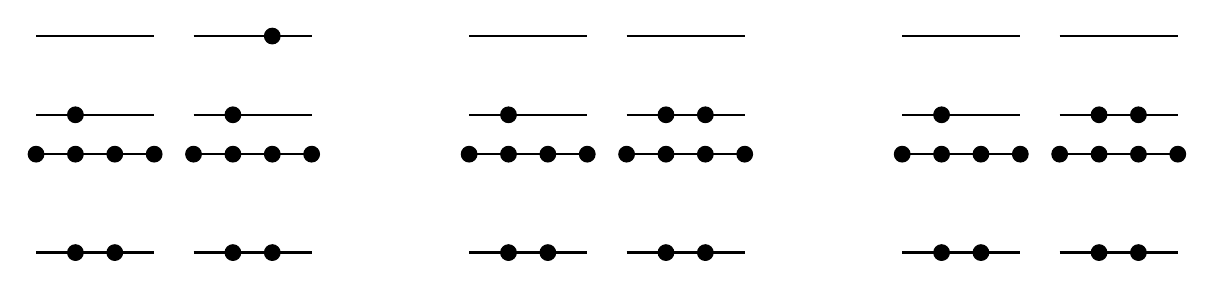
\begin{tikzpicture}
        \foreach \x in {0.5, 2.5, 6, 8, 11.5, 13.5}{
            \foreach \y in {0, 1.25, 1.75, 2.75}{
                \draw [thick] (\x, \y) -- ++(1.5, 0);
            }
            \node[draw, circle, inner sep=2pt, fill] at (\x+0.5, 0){};
            \node[draw, circle, inner sep=2pt, fill] at (\x+1, 0)(1.5,0){};
            \node[draw, circle, inner sep=2pt, fill] at (\x, 1.25){};
            \node[draw, circle, inner sep=2pt, fill] at (\x+0.5, 1.25){};
            \node[draw, circle, inner sep=2pt, fill] at (\x+1, 1.25){};
            \node[draw, circle, inner sep=2pt, fill] at (\x+1.5, 1.25){};
            \node[draw, circle, inner sep=2pt, fill] at (\x+0.5, 1.75){};
        }
        \node[draw, circle, inner sep=2pt, fill] at (3.5, 2.75){};
        \node[draw, circle, inner sep=2pt, fill] at (9, 1.75){};
        \node[draw, circle, inner sep=2pt, fill] at (14.5, 1.75){};
    \end{tikzpicture}
    \caption{nothing}
    \label{fig:nitrogen_nucleons_states}
\end{figure}